\documentclass{article}
\usepackage[utf8]{inputenc}
\usepackage[a4paper,hmargin =1.2 in,bottom =1.5in]{geometry}
\usepackage[parfill]{parskip}
\usepackage{hyperref}
\usepackage{fancyhdr}
\usepackage{enumitem}
\usepackage{amsmath}
\usepackage{amsthm}
\usepackage{amssymb}
\usepackage[linesnumbered,ruled,vlined]{algorithm2e}
\usepackage{listings}
\usepackage{xcolor}
\usepackage{floatrow}
\usepackage{graphicx}
\usepackage{caption}
\usepackage{subcaption}

\pagestyle{fancy}
\fancyhf{}
\lhead{
    200020012 and 200050093
}
\rhead{
    CS736 Assignment 2
}
\cfoot{Page \thepage}
\renewcommand{\footrulewidth}{1pt}
\pagestyle{empty} 

\newtheorem{definition}{Definition}

\begin{document}
\title{CS736 Assignment 2}
\author{Adish Shah and Padakanti Akshay Kiran}
\date{March 2022}
\maketitle
\thispagestyle{empty}
\tableofcontents
\newpage
\thispagestyle{fancy}




\section{Problem 1}
\subsection{d) Initial Pointsets}
\begin{figure}[H]
    \centerline{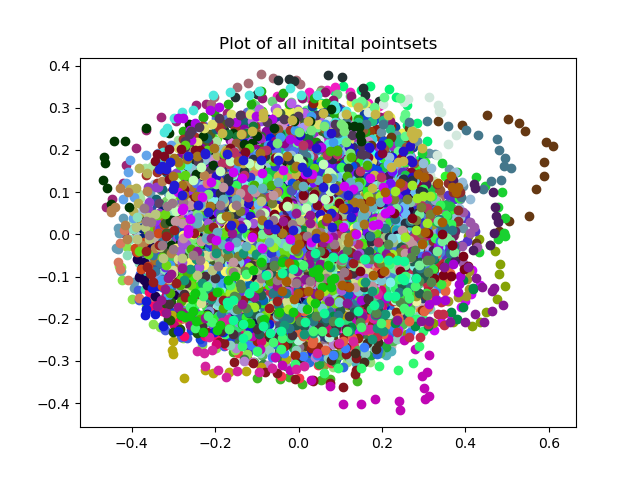
\includegraphics[scale=0.5]{../results/ellipses/initial-all-data-scatter.png}}
    \caption{Scatter plot}
\end{figure}

\begin{figure}[H]
    \centerline{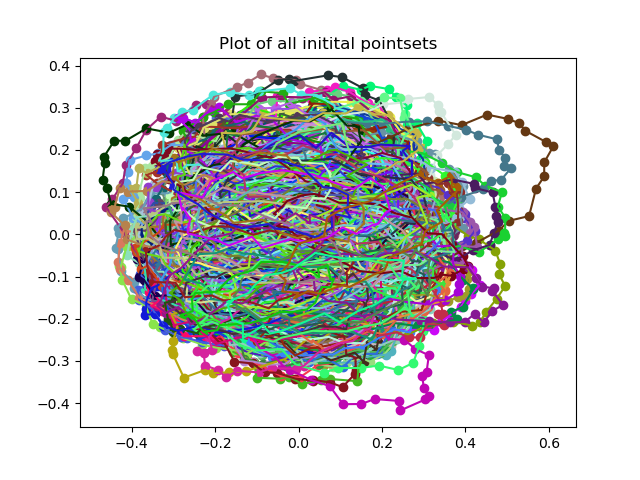
\includegraphics[scale=0.5]{../results/ellipses/initial-all-data-polyline.png}}
    \caption{Each pointset represented by polylines}
\end{figure}

\newpage
\thispagestyle{fancy}
\subsection{e)}
\begin{figure}[H]
    \centerline{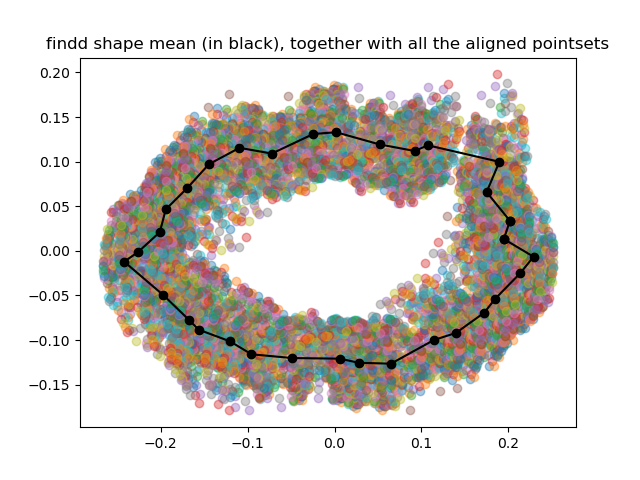
\includegraphics[scale=0.5]{../results/ellipses/mean-and-aligned-data.png}}
    \caption{Result based on code11}
\end{figure}

\begin{figure}[H]
    \centerline{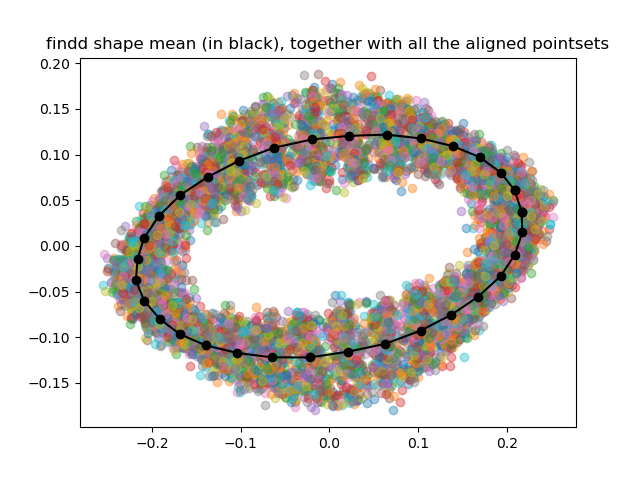
\includegraphics[scale=0.5]{../results/ellipses/mean-and-aligned-data2.png}}
    \caption{Result based on code22}
\end{figure}

\newpage
\thispagestyle{fancy}

\subsection{f)}
\begin{figure}[H]
    \centerline{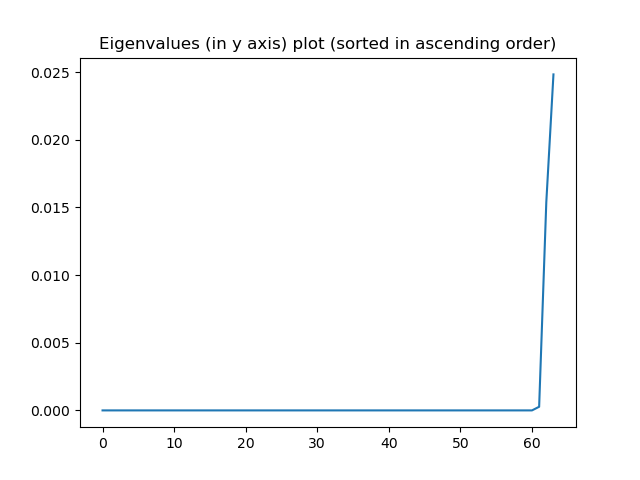
\includegraphics[scale=0.5]{../results/ellipses/eigen-values.png}}
    \caption{Result based on code11. First two eigenvalues are significantly greater than other eigenvalues which are close to 0}
\end{figure}

\begin{figure}[H]
    \centerline{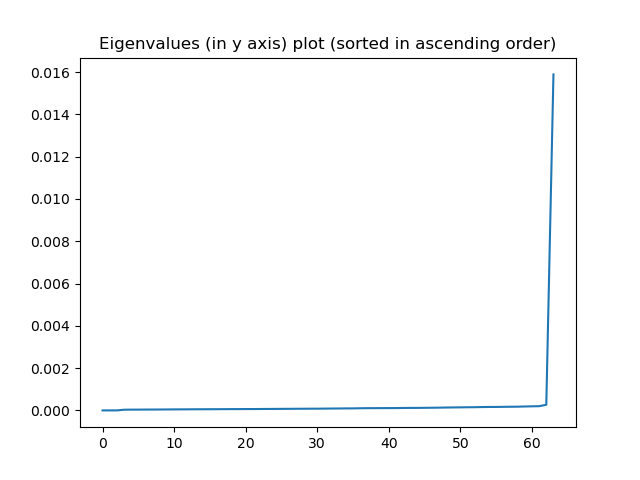
\includegraphics[scale=0.5]{../results/ellipses/eigen-values2.png}}
    \caption{Result based on code22}
\end{figure}

\newpage
\thispagestyle{fancy}

\subsection{g)}
\subsubsection{Results based on code11}
\begin{figure}[H]
    \centerline{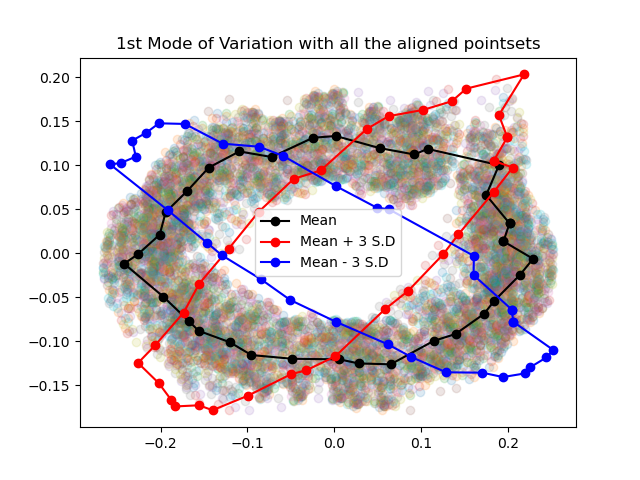
\includegraphics[scale=0.45]{../results/ellipses/mean-and-first-mode.png}}
    \caption{First Mode of variation}
\end{figure}

\begin{figure}[H]
    \centerline{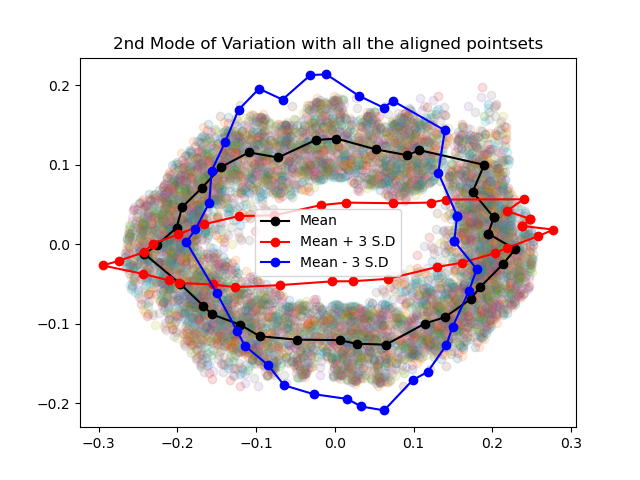
\includegraphics[scale=0.45]{../results/ellipses/mean-and-second-mode.png}}
    \caption{Second Mode of variation}
\end{figure}

\begin{figure}[H]
    \centerline{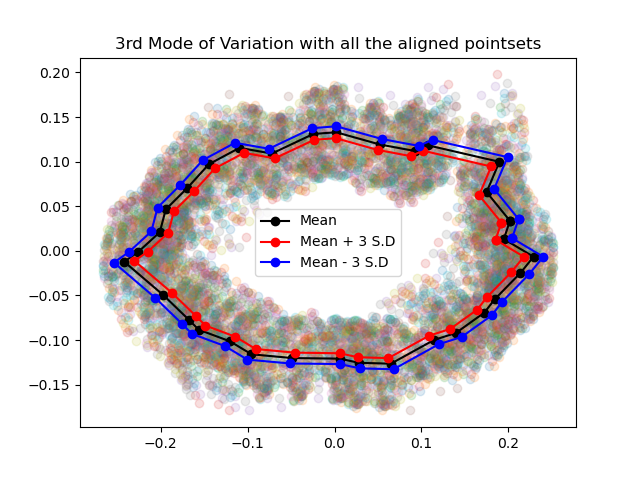
\includegraphics[scale=0.45]{../results/ellipses/mean-and-third-mode.png}}
    \caption{Third mode of variation}
\end{figure}

\newpage
\thispagestyle{fancy}

\subsubsection{Results based on code22}
\begin{figure}[H]
    \centerline{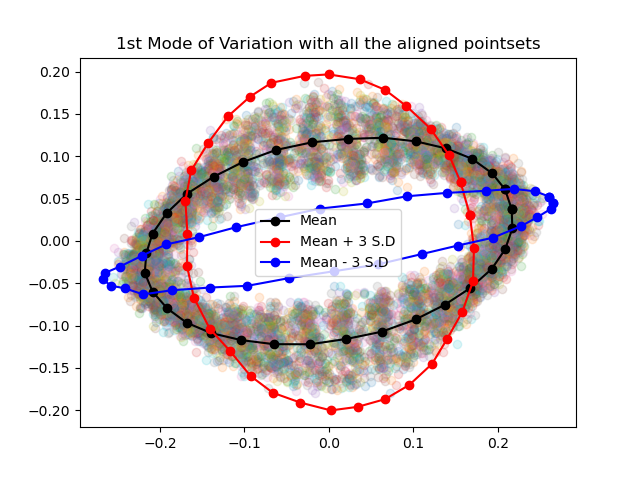
\includegraphics[scale=0.45]{../results/ellipses/mean-and-first-mode_2.png}}
    \caption{First Mode of variation}
\end{figure}

\begin{figure}[H]
    \centerline{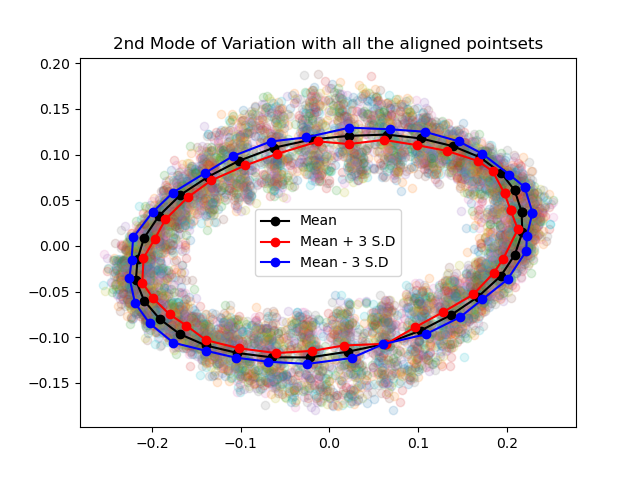
\includegraphics[scale=0.45]{../results/ellipses/mean-and-second-mode_2.png}}
    \caption{Second Mode of variation}
\end{figure}

\begin{figure}[H]
    \centerline{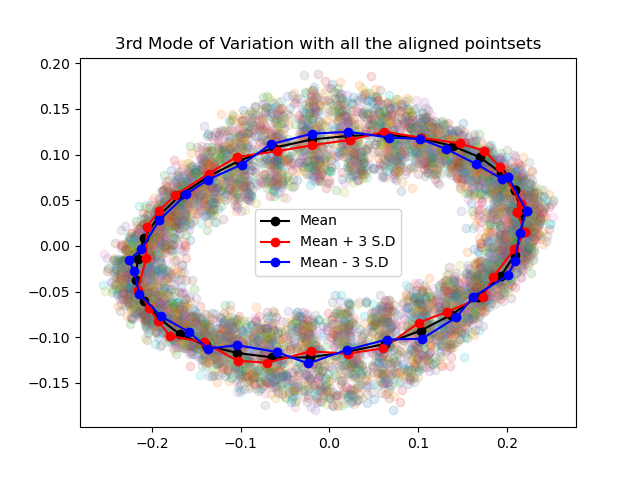
\includegraphics[scale=0.45]{../results/ellipses/mean-and-third-mode_2.png}}
    \caption{Third mode of variation}
\end{figure}

\section{Problem 2}

\subsection{d) Initial Pointsets}
\begin{figure}[H]
    \centerline{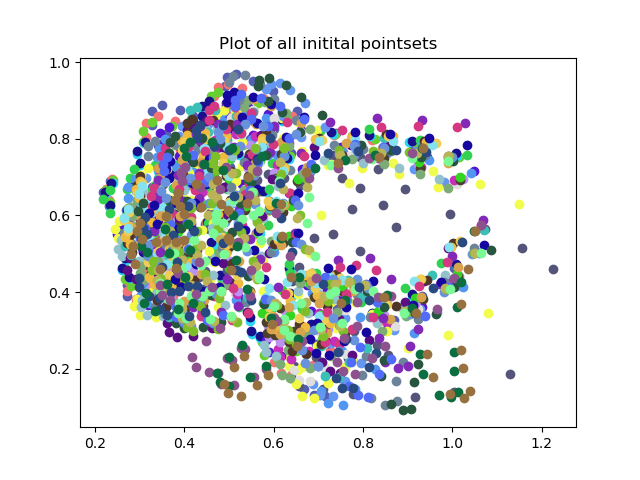
\includegraphics[scale=0.5]{../results/hand/initial-all-data-scatter.png}}
    \caption{Scatter plot}
\end{figure}

\begin{figure}[H]
    \centerline{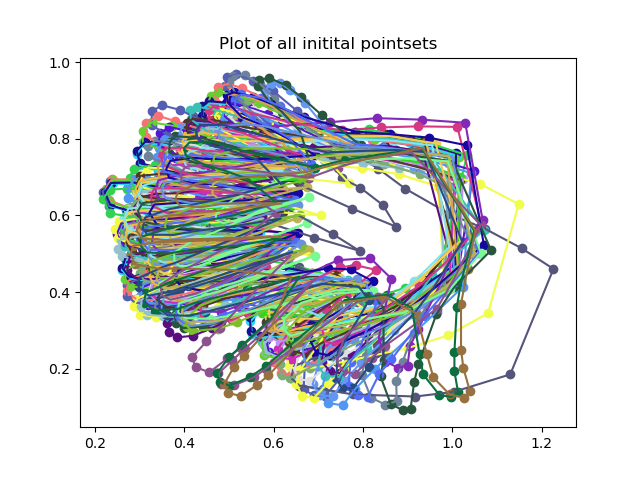
\includegraphics[scale=0.5]{../results/hand/initial-all-data-polyline.png}}
    \caption{Each pointset represented by polylines}
\end{figure}

\newpage
\thispagestyle{fancy}

\subsection{e)}
\begin{figure}[H]
    \centerline{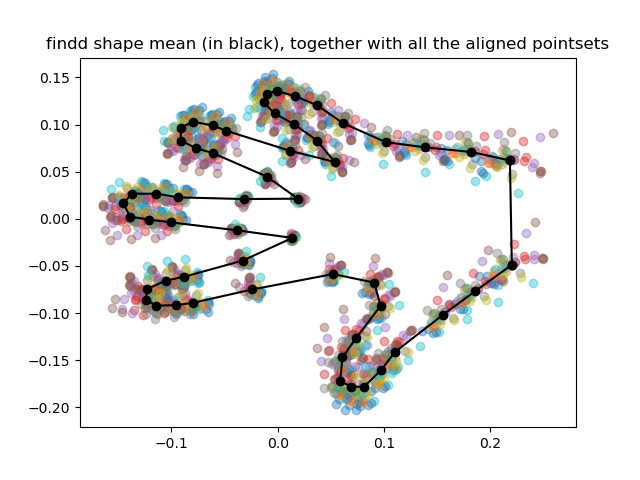
\includegraphics[scale=0.5]{../results/hand/mean-and-aligned-data.png}}
    \caption{Result based on code11}
\end{figure}

\begin{figure}[H]
    \centerline{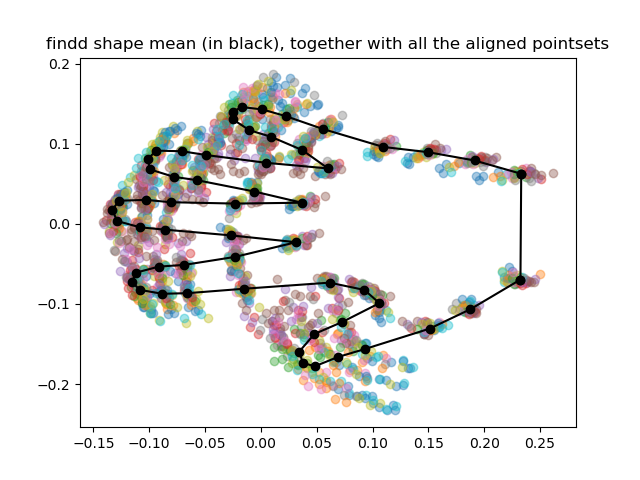
\includegraphics[scale=0.5]{../results/hand/mean-and-aligned-data2.png}}
    \caption{Result based on code22}
\end{figure}

\newpage
\thispagestyle{fancy}

\subsection{f)}
\begin{figure}[H]
    \centerline{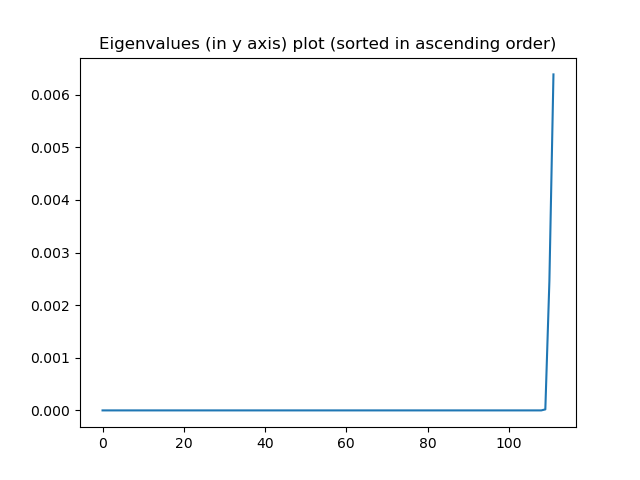
\includegraphics[scale=0.5]{../results/hand/eigen-values.png}}
    \caption{Result based on code11. First two eigenvalues are significantly greater than other eigenvalues which are close to 0}
\end{figure}

\begin{figure}[H]
    \centerline{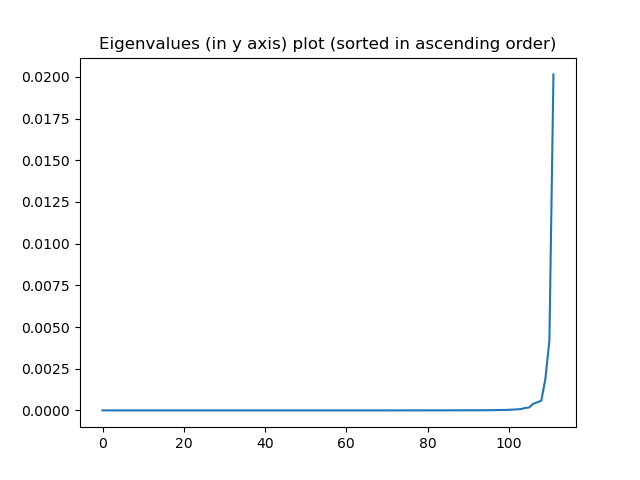
\includegraphics[scale=0.5]{../results/hand/eigen-values2.png}}
    \caption{Result based on code22}
\end{figure}

\newpage
\thispagestyle{fancy}

\subsection{g)}
\subsubsection{Results based on code11}
\begin{figure}[H]
    \centerline{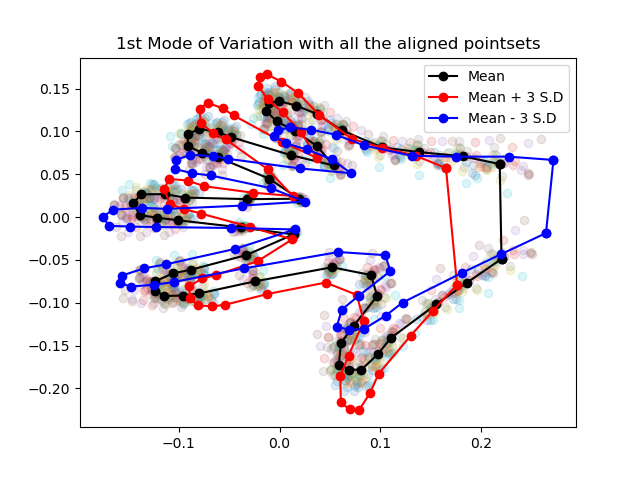
\includegraphics[scale=0.45]{../results/hand/mean-and-first-mode.png}}
    \caption{First Mode of variation captures}
\end{figure}

\begin{figure}[H]
    \centerline{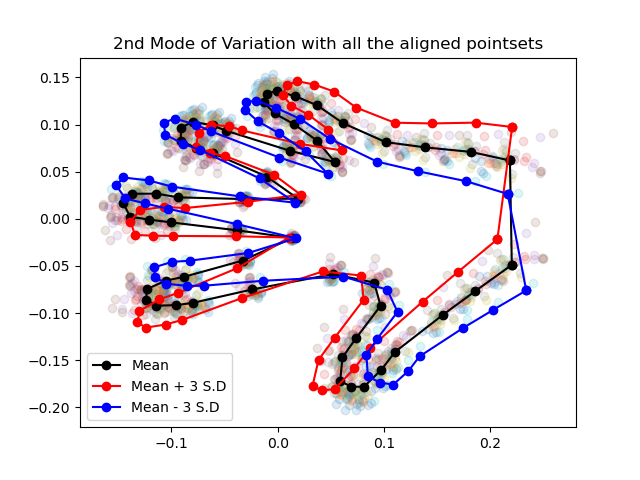
\includegraphics[scale=0.45]{../results/hand/mean-and-second-mode.png}}
    \caption{Second Mode of variation}
\end{figure}

\begin{figure}[H]
    \centerline{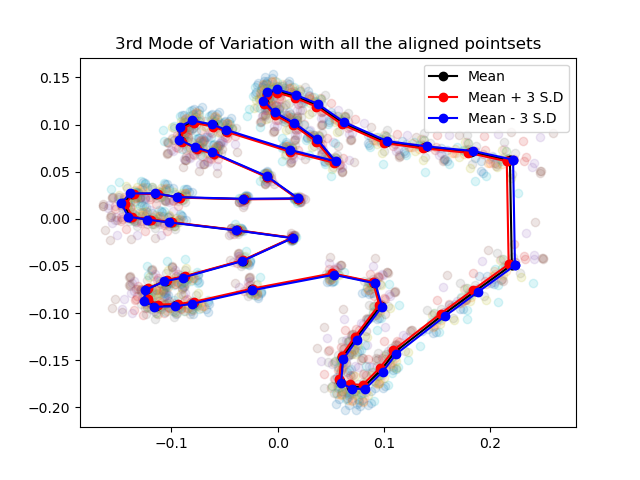
\includegraphics[scale=0.45]{../results/hand/mean-and-third-mode.png}}
    \caption{Third mode of variation}
\end{figure}

\newpage
\thispagestyle{fancy}

\subsubsection{Results based on code22}
\begin{figure}[H]
    \centerline{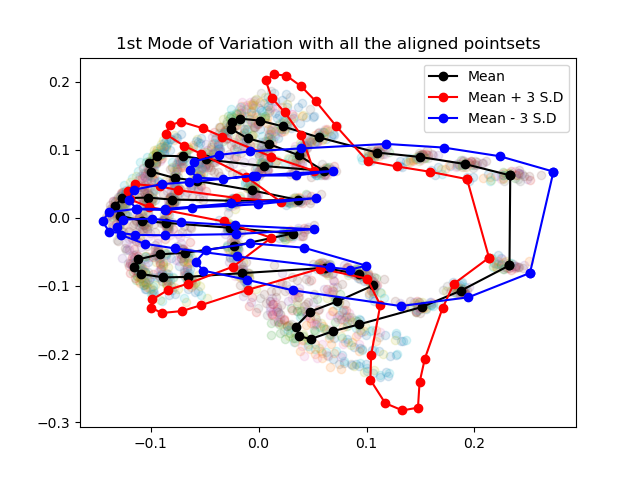
\includegraphics[scale=0.45]{../results/hand/mean-and-first-mode_2.png}}
    \caption{First Mode of variation }
\end{figure}

\begin{figure}[H]
    \centerline{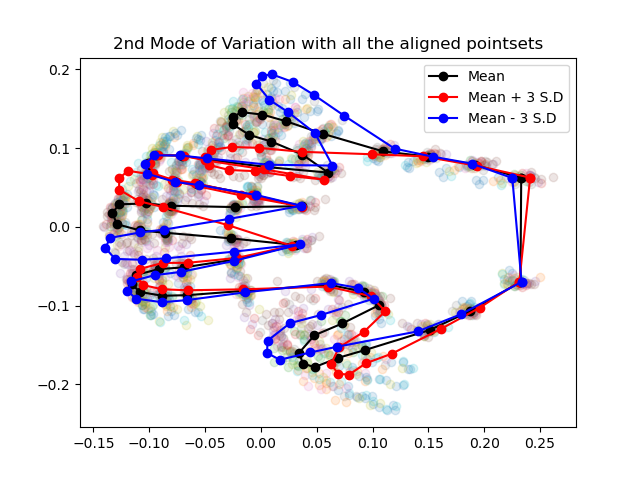
\includegraphics[scale=0.45]{../results/hand/mean-and-second-mode_2.png}}
    \caption{Second Mode of variation}
\end{figure}

\begin{figure}[H]
    \centerline{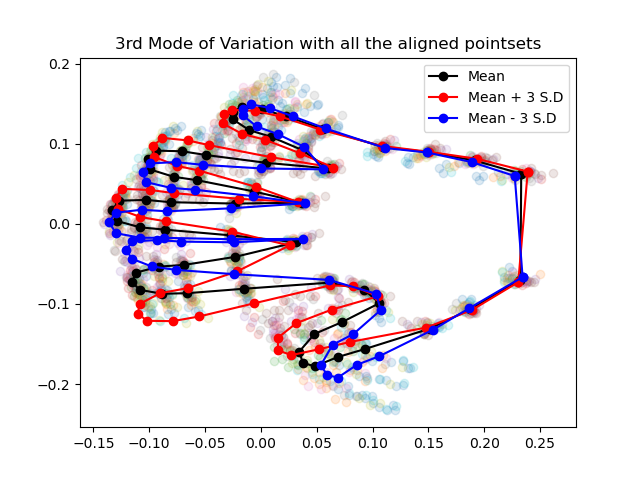
\includegraphics[scale=0.45]{../results/hand/mean-and-third-mode_2.png}}
    \caption{Third mode of variation}
\end{figure}



\newpage
\thispagestyle{fancy}
\section{Problem 3}


\subsection{Procrustes Distance}
The simplest way to define proximity is just the magnitude of the Euclidean norm of the difference between the two shape vectors in $\mathbb{R}^{dN}$ which is the square of the Procrustes distance between the shapes.
Procrustes distance between $z_{1}$ and $z_{2}$ (resulting from aligning $z_{2}$ to $z_{1}$ by similarity transformations is 
$$min_{\theta,T,s} \sum_{n = 1,...,N} || z_{1n} - s M_{\theta} z_{2n} - T ||$$
where s is the scaling factor, $M_{\theta}$ is the rotation matrix of dimensions $d \times d$ and T represents a translation in $\mathbb{R}^{d}$.
\subsection{K - means algorithm in the Shape space}
We apply the k-means algorithm to the points $X_{1}, X_{2}, \dots,X_{n}$ by using the Procrustes distance and Procrustes Mean.

\subsection{Objective Function}
$$W(\mathcal{C},[Z_{1}], \dots, [Z_{k} ]) = \sum_{i=1}^{k} \sum_{l \in C_{i}} Procrustes\_distance([X_{l}],[Z_{i}])$$
\subsection{Algorithm for clustering}
\begin{enumerate}
    \item \textbf{Initialisation condition} The starting centroid vector can be assigned in different ways: at random, using prior information,
    etc. In our application we will choose it at random.
    \item Given a vector of shapes $Z = ([Z_{1}], \dots, [Z_{k} ]) \; \; [Z_{i}] \in \sum_{3}^{n} \; \; i = 1, . . . , k$ we minimize
    with respect to $\mathcal{C} = (C_{1},\dots, C_{k} ) $ assigning each shape
    $([X_{1}],\dots, [X_{n}])$ to the class whose centroid has the minimum Procrustes distance to it.
    \item Given $\mathcal{C}$, we minimize with respect to the vector shapes $Z$, taking $Z = ([\hat{\mu_{1}}],\dots, [\hat{\mu_{k}}])$,
    and $[\hat{\mu_{i}}] \;\; i = 1, . . . , k$ , the Procrustes mean of shapes in $C_{i}$. This is calculated using the algorithm mentioned below.
    \item Repeat steps 2 and 3 till convergence.
    \item \textbf{Stopping condition} When the value of the objective function doesn't decrease further, we stop.
\end{enumerate}


\subsection{Algorithm to find the Procrustes Means}
\begin{enumerate}
    \item Center the configurations to remove location. Let $X_{i}, i = 1, \dots,n $ be the configurations. Initially let 
    \[X_{i}^{P} = X_{i}, i = 1, \dots,n  \]
    \item Calculate $G = \frac{1}{n} \sum_{i=1}^{n-1} \sum_{j = i+1}^{n} ||X_{i}^{P} - X_{j}^{P}||^{2}$
    For the $i$th configuration let 
    \[\overline{X}_{(i)} = \frac{1}{n-1} \sum_{j \neq i} X_{i}^{P}\]
    We can optimise $|| \overline{X}_{(i)} - X_{i}^{P}M||^{2}$ over rotations.
    Set $X_{i}^{P} = X_{i}^{P}\hat{M}$, where $\hat{M}$ is the optimal rotation matrix. Repeat this for all i.
    Calculate the new G value. This process is repeated until G can't be reduced further.
    \newpage
    \thispagestyle{fancy}
    \item For the $i$th configuration calculate $\hat{\beta_{i}} = \frac{\sum_{k=1}^{n} ||X_{k}^{P}||^{2}}{||X_{i}^{P}||^{2}}^{1/2} \phi_{i}$, 
    where $\phi_{i}$ is the $i$th component  of the eigenvector $\phi$ corresponding to the largest eigenvalue of the correlation
    matrix $\phi$ of the $vector(X_{i}^{P})$.
    Set $X_{i}^{P} = \hat{\beta_{i}}X_{i}^{P}$. Repeat this for all i and calculate the new G value.
    \item Repeat steps 2 and 3 until G cannot be reduced further.
    \item \[ [\hat{\mu}] = \frac{1}{n} \sum_{i}^{n} X_{i}^{P}\]
\end{enumerate}
\end{document}
